%!TeX program = XeLaTex
%!TEX encoding = UTF-8 Unicode

\documentclass[10pt,twoside]{book}
\XeTeXlinebreaklocale "my_MM"  %Myanmar line and character breaks
\XeTeXinterwordspaceshaping=2

\usepackage[
    paperheight = 10.2in,
    paperwidth = 7.4in,
    right = 0.8in,
    left = 1.45in,
    top = 0.75in,
    bottom = 0.9in,
    heightrounded,
    asymmetric,
    %showframe
]{geometry}
\usepackage[parfill,indent=2em,skip=3pt plus 1pt]{parskip}
\usepackage{bm}

\usepackage{fontspec}

\usepackage{titlesec}
\usepackage{fancyhdr}

\usepackage[dvipsnames]{xcolor}
\usepackage{siunitx}

\usepackage{caption}
\usepackage[labelformat=simple]{subcaption}

\usepackage[textcolor=blue,
    textsize=scriptsize,
    textwidth=17.5mm,
    color=red!25,
    disable]{todonotes}

\usepackage{booktabs}
\usepackage{array}

\usepackage{amsmath}
\usepackage{mathtools}

\usepackage{afterpage}
\usepackage{adjustbox}

\usepackage{tikz}
\usepackage{tikz-3dplot}

\newcommand\blankpage{%
    \null
    \thispagestyle{empty}%
    \addtocounter{page}{-1}%
    \newpage}

\input{preamble/font}
\input{preamble/page_style}

\pagestyle{fancy}

\begin{document}
\chapter{Introduction to Vectors} \label{ch:ch01}

\section{Vectors and Linear Combinations}
\subsection*{ဗက်တာ (Vector)}
\fEn{“What is a vector?”} ဗက်တာဆိုတာ ဘာလဲ။ ဒီမေးခွန်းကို မဖြေခင်မှာ ကိန်းစစ် \fEn{(real numbers)} တွေနဲ့ ဖွဲ့စည်းထားတဲ့ ဗက်တာ ဥပမာတချို့ကို ကြည့်ရအောင်။ 

\[
\begin{bmatrix*}[r] 1\\ 3\\ \end{bmatrix*}, \qquad
\begin{bmatrix*}[r] -1\\ 3\\ \end{bmatrix*}, \qquad
\begin{bmatrix*}[r] 1.5\\ -3.2\\ \end{bmatrix*}
\]

\[
\begin{bmatrix*}[r] 3\\ 3\\ 2\\\end{bmatrix*}, \qquad
\begin{bmatrix*}[r] -1\\ 3\\ 1\\\end{bmatrix*}, \qquad
\begin{bmatrix*}[r] 1.5\\ 1\\ \sqrt{2}\end{bmatrix*}
\]
ပထမသုံးခုဟာ \fEn{2-dimensional} ဗက်တာတွေပါ။ ဒုတိယသုံးခုကတော့ \fEn{3-dimensional} တွေဖြစ်ပါတယ်။ ဗက်တာတစ်ခုမှာ ကိန်းဂဏန်း တစ်လုံးနဲ့အထက် ပါဝင်နိုင်ပြီး လေးထောင့်ကွင်းထဲမှာ ကော်လံတစ်ခုအနေနဲ့ အထက်အောက်စီ ရေးလေ့ရှိတယ်။ ပါဝင်တဲ့ ကိန်းတစ်ခုချင်းစီကို \fEnEmpBf{component} တွေလို့ခေါ်ပါတယ်။ ဘယ်လောက် \fEn{dimensional} ဗက်တာ ဖြစ်တယ်ဆိုတာကို ပါဝင်တဲ့ \fEnEmp{component} အရေအတွက်နဲ့ ခွဲခြားသတ်မှတ်တာ။ \fEn{Component} လေးခုပါရင် \fEn{4-dimensional,} \fEnEmpBf{n} ခုပါတဲ့အခါ \fEnEmpBf{n-dimensional} ဗက်တာခေါ်တာပေါ့။

\fEn{n-dimensional} ဗက်တာတွေ အားလုံးပါဝင်တဲ့ အစုကို \fEnEmpBf{Euclidean n-space} လို့ ခေါ်ပါတယ်။ ဥပမာအားဖြင့် \fEn{2-space} ဟာ \fEn{2-dimensional} ဗက်တာတွေ အားလုံးပါဝင်တဲ့ အစု၊ \fEn{3-space} ဟာ \fEn{3-dimensional} ဗက်တာတွေ အားလုံးပါဝင်တဲ့ အစု ဖြစ်ပါတယ်။ 

\fEn{Real number} တွေ အနန္တရှိကြတယ်။ \fEn{Real number} တွေနဲ့ ဖွဲ့စည်းထားတဲ့ \fEn{2-dimensional} ဗက်တာတွေလည်း အနန္တရှိကြရမယ်။ \fEn{3-dimensional} တွေလည်း ထိုနည်းလည်းကောင်းပါပဲ။ ဒါကြောင့် \fEn{n-space} တစ်ခုမှာ အနန္တများပြားတဲ့ ဗက်တာတွေ ပါဝင်နေမှာဖြစ်တယ်။ 

ဗက်တာတွေကို \(\vec{u}, \vec{v}, \vec{w}\) စတဲ့ အင်္ဂလိပ်အက္ခရာ အပေါ်မှာ မြှားလေးတင်ထားတဲ့ သင်္ကေတလေးတွေနဲ့ ကိုယ်စားပြုဖော်ပြလေ့ရှိတယ်။
\[
\vec{v} = \begin{bmatrix*}[r] 1\\ 2\\ \end{bmatrix*}, \qquad
\vec{v} = \begin{bmatrix*}[r] -1\\ 3\\ 3\\\end{bmatrix*}, \qquad
\vec{w} = \begin{bmatrix*}[r] 1.5\\ -3.2\\ \sqrt{2}\\ \sqrt{3}\\\end{bmatrix*}
\]
ဗက်တာ \fEn{component} တွေကိုတော့ အခုလို သင်္ကေတနဲ့ ဖော်ပြလေ့ရှိတယ်။ \fEn{Component} တွေဟာ သာမန် ဂဏန်းတွေပဲဖြစ်တဲ့အတွက် ၎င်းတို့ကို ကိုယ်စားပြုတဲ့အခါ မြှားမသုံးပါဘူး။
\[
\vec{v} = \begin{bmatrix*}[r] v_{1} \\ v_{2} \\ \end{bmatrix*}, \qquad
\vec{w} = \begin{bmatrix*}[r] w_{1} \\ w_{2} \\ w_{3} \\ \end{bmatrix*}, \qquad
\]
\(\vec{v} = \begin{bsmallmatrix*}[r] 2 \\ 3\\ \end{bsmallmatrix*}\) ဖြစ်ရင် $v_{1}=2, v_{2}=3$ ဖြစ်တယ်။

\subsection*{ဗက်တာ ပေါင်းခြင်းနှင့် စကေလာဖြင့် မြှောက်ခြင်း}
ဗက်တာ အော်ပရေးရှင်းနှစ်ခုရှိတယ်။ ပထမတစ်ခုက ဗက်တာ ပေါင်းခြင်း \fEn{(Vector Addition)}။  ဗက်တာအချင်းချင်း ပေါင်းတာကို အခုလို သတ်မှတ်ပါတယ်။ \fEn{Dimension} တူရပါမယ်။
%
\[
\vec{u} = \begin{bmatrix*}[r] 4\\ 2\\ \end{bmatrix*}, \qquad
\vec{v} = \begin{bmatrix*}[r] -1\\ 2\\ \end{bmatrix*}, \qquad
\vec{u} + \vec{v} = \begin{bmatrix*}[r] 4\\ 2\\ \end{bmatrix*} +  \begin{bmatrix*}[r] -1\\ 2\\ \end{bmatrix*} = \begin{bmatrix*}[r] 3\\ 4\\ \end{bmatrix*}
\]
%
လိုက်ဖက် \fEn{component} အချင်းချင်း ပေါင်းပေးရတာပါပဲ။ ပေါင်းလဒ်ဟာ ဗက်တာတစ်ခုပဲ ဖြစ်ပြီး \fEn{dimension} လည်း အတူတူပဲဖြစ်တယ်။ ဗက်တာတွေ နှုတ်လို့လည်းရတာပေါ့။ 
%
\[
\vec{u} - \vec{v} = \begin{bmatrix*}[r] 4\\ 2\\ \end{bmatrix*} -  \begin{bmatrix*}[r] -1\\ 2\\ \end{bmatrix*} = \begin{bmatrix*}[r] 5\\ 0\\ \end{bmatrix*}
\]
%

ဒုတိယ ဗက်တာ အော်ပရေးရှင်းကတော့ စကေလာဖြင့်မြှောက်ခြင်း \fEn{(Scalar Multiplication)} ပါ။ ဒီလိုသတ်မှတ်ပါတယ်။
%
\[
\vec{u} = \begin{bmatrix*}[r] 4\\ 2\\ \end{bmatrix*},\qquad
\vec{v} = \begin{bmatrix*}[r] -1\\ 2\\ \end{bmatrix*},\qquad
2\vec{u}= 2\begin{bmatrix*}[r] 4\\ 2\\ \end{bmatrix*} = \begin{bmatrix*}[r] 8\\ 4\\ \end{bmatrix*},\qquad
-2.5\vec{v}= -2.5 \begin{bmatrix*}[r] -1\\ 2\\ \end{bmatrix*} = \begin{bmatrix*}[r] 2.5\\ -5\\ \end{bmatrix*}
\]
%
ဗက်တာတစ်ခုကို ရိုးရိုးဂဏန်းတစ်ခုနဲ့ မြှောက်တာပါပဲ။ \fEn{Component} တစ်ခုချင်းကို မြှောက်ပေးရတယ်။ ရလဒ်ဟာ ဗက်တာတစ်ခုဖြစ်ပြီး \fEn{dimension} မပြောင်းလဲဘူး။

\subsection*{Linear Combinations}
ဗက်တာပေါင်းခြင်းနဲ့ စကေလာဖြင့်မြှောက်ခြင်း နှစ်ခုပေါင်းစည်းထားတာကို \fEnEmpBf{Linear Combinations} လို့ခေါ်တာပါ။ ဥပမာ
%
\[
2 \begin{bmatrix*}[r] 4\\ 2\\ \end{bmatrix*} 
                        + -2.5 \begin{bmatrix*}[r] -1\\ 2\\ \end{bmatrix*} 
                        = \begin{bmatrix*}[r] 8\\ 4\\ \end{bmatrix*} 
                            + \begin{bmatrix*}[r] 2.5\\ -5\\ \end{bmatrix*}
                        = \begin{bmatrix*}[r] 10.5\\ -1\\ \end{bmatrix*}
\]
%
%
\[
3 \begin{bmatrix*}[r] 1\\ 3\\ 5\\\end{bmatrix*} 
                        + -1 \begin{bmatrix*}[r] 2\\ 4\\ 6\\\end{bmatrix*} 
                        = \begin{bmatrix*}[r] 3\\ 9\\ 15\\\end{bmatrix*} 
                            + \begin{bmatrix*}[r] -2\\ -5\\ -6\\\end{bmatrix*}
                        = \begin{bmatrix*}[r] 1\\ 4\\ 9\\\end{bmatrix*}
\]
%
ဗက်တာ $\vec{u}$ နဲ့  $\vec{v}$ တို့ရဲ့ \fEn{linear combinations} ကို 
\[
c\vec{u} + d\vec{v}    
    \]
အဖြစ် အဓိပ္ပါယ်သတ်မှတ်တယ်။ $c$ နဲ့ $d$ ဟာ ကိန်းစစ်တွေဖြစ်ပြီး စကေလာ \fEn{(scalar)} တွေလို့ခေါ်ပါတယ်။ ဗက်တာနဲ့ စကေလာ မရောထွေးရပါဘူး။ $2$ ဟာ စကေလာဖြစ်ပြီး \(\begin{bsmallmatrix*}[r] 2\\\end{bsmallmatrix*}\) ကတော့ \fEn{1-dimensional} ဗက်တာပါ။

$c = d = 1$ ဖြစ်ရင် ဗက်တာနှစ်ခု ပေါင်းတာပဲဖြစ်တဲ့အတွက် ဗက်တာပေါင်းခြင်းကို \fEn{linear combinations}  ရဲ့ \fEn{special case} တစ်ခုလို့ ရှုမြင်နိုင်တယ်။
%
\[
1\vec{u} + 1\vec{v} =  \vec{u} + \vec{v} 
    \]
%
ဗက်တာနှုတ်ခြင်းကိုလည်း \fEn{linear combinations}  ရဲ့ \fEn{special case} တစ်ခုလို့ ရှုမြင်နိုင်တယ်။ $c = 1, d = -1$ ဖြစ်ရင် \fEn{linear combination} ဟာ ဗက်တာနှစ်ခု နှုတ်တာပါပဲ။
%
\[
1\vec{u} + -1\vec{v} =  1\vec{u} - 1\vec{v} = \vec{u} - \vec{v}
    \]
%
စကေလာဖြင့်မြှောက်ခြင်းကိုလည်း \fEn{linear combinations}  ရဲ့ \fEn{special case} တစ်ခုလို့ ရှုမြင်နိုင်တယ်။ $c = 0$ သို့မဟုတ် $d = 0$ ဖြစ်တဲ့အခါမှာ
%
\[
c\vec{u} + 0\vec{v} =  c\vec{u} + \vec{0} = c\vec{u}
    \]
\[
0\vec{u} + d\vec{v} =  \vec{0} + d\vec{v} = d\vec{v}
    \]
%
မှတ်ချက်။\qquad ။ \fEn{Component} အားလုံး သုညဖြစ်တဲ့ ဗက်တာတွေကို သုညဗက်တာ \fEn{(\textbf{\textit{zero vector}})} လို့ခေါ်ပြီး $\vec{0}$ နဲ့ကိုယ်စားပြုပါတယ်။ မည်သည့်ဗက်တာကိုမဆို သုညနဲ့ မြှောက်တဲ့အခါ ရလဒ်ဟာ \fEn{\textit{zero vector}} ဖြစ်ပြီး \fEn{\textit{zero vector}} ကို မည်သည့် စကေလာဖြင့် မြှောက်သည်ဖြစ်စေ ရလဒ်ဟာ \fEn{\textit{zero vector}} ပဲဖြစ်ပါမယ်။ 
%
\[\begin{bmatrix*}[r] 0\\ 0\\\end{bmatrix*}, \qquad
\begin{bmatrix*}[r] 0\\ 0\\ 0\\\end{bmatrix*}, \qquad
0\begin{bmatrix*}[r] 1\\ 2\\ -2\\\end{bmatrix*} = 
    \begin{bmatrix*}[r] 0\\ 0\\ 0\\\end{bmatrix*}, \qquad
c\begin{bmatrix*}[r] 0\\ 0\\ 0\\\end{bmatrix*} = \begin{bmatrix*}[r] 0\\ 0\\ 0\\\end{bmatrix*} \fEn{ (for any real } c)\] 
%

$c = 0$ နဲ့ $d = 0$ ဖြစ်လို့ရတဲ့အတွက် \fEn{linear combinations} ဖြင့် \fEn{\textit{zero vector}} ကို အမြဲရရှိနိုင်တယ်ဆိုတာ အထူးဂရုပြု မှတ်သားထားသင့်ပါတယ်။ မြှောက်ဖော်ကိန်း \fEn{coefficient} နှစ်ခုကို ($c$ နဲ့ $d$ ကို ဆိုလို) သုညထားလိုက်တဲ့အခါ \fEn{\textit{zero vector}} ရတာပေါ့။
\[0\vec{u} + 0\vec{v} = \vec{0} \quad (\fEn{for any n-dimensional $\vec{u}$ and $\vec{v}$})\]

\subsection*{ဗက်တာများကို ပုံဖော်ကြည့်ခြင်း}
\fEn{2-dimensional} ဗက်တာတွေကို ပုံဖော်ကြည့်ဖို့ စံသုံးနေကြ \fEn{\textit{xy}-plane} ကို အသုံးပြုနိုင်ပါတယ်။ ဗက်တာ $\vec{v} = \begin{bsmallmatrix*}[r] 4\\ 2\\\end{bsmallmatrix*}$ ကို $(0, 0)$ ကနေ $(4, 2)$ အမှတ်ထိ အလျားရှိတဲ့ မြှားနဲ့ ဖော်ပြပါတယ်။ ထိုနည်းတူစွာ $\vec{w} = \begin{bsmallmatrix*}[r] -1\\ 2\\\end{bsmallmatrix*}$ ကို $(0, 0)$ ကနေ $(-1, 2)$ အမှတ်ထိ အလျားရှိတဲ့ မြှားနဲ့ ဖော်ပြတယ်။ မြှားအမြီးဟာ \fEnEmpBf{origin} $(0, 0)$ မှစပြီး မြှားခေါင်းကတော့ ဗက်တာရဲ့ \fEn{components} နှစ်ခုနဲ့ လိုက်ဖက်တဲ့ $(x, y)$ ကိုသြဒိနိတ် အမှတ်မှာဆုံးရပါမယ်။

\hspace*{-0.5cm}
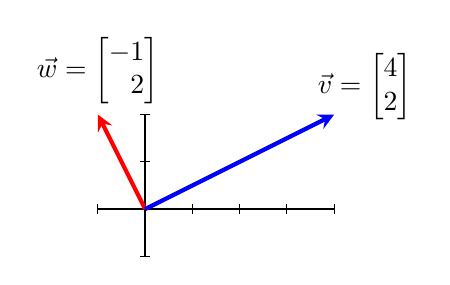
\begin{tikzpicture}[scale=0.6]
    % X and YAxis
    \draw[semithick] (-1,0) -- (4,0);
    \draw[semithick] (0,-1) -- (0,2);
    % Ticks
    \foreach \x in {-1,0,...,4} {%
        \draw ($(\x,0) + (0,-0.1)$) -- ($(\x,0) + (0,0.1)$);
    }
    \foreach \y in {-1,...,2} {%
        \draw ($(0,\y) + (-0.1,0)$) -- ($(0,\y) + (0.1,0)$);
    }
    % Vectors
    \draw[line width=1.5pt,-stealth, red](0,0)--(-1,2) node[anchor=south,text=black]{$\vec{w} = \begin{bmatrix*}[r] -1\\   2\\\end{bmatrix*}$};
    \draw[line width=1.5pt,-stealth,blue](0,0)--(4,2) node[xshift=-1em,yshift=1em, anchor=west,text=black]{$\vec{v} = \begin  {bmatrix*}[r] 4\\ 2\\\end{bmatrix*}$};
\end{tikzpicture}

%
\begin{figure}[htb!]   
    \hspace*{-2mm}
    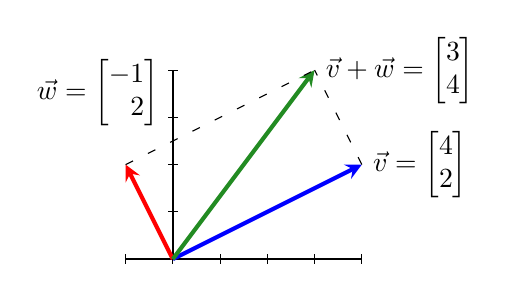
\begin{tikzpicture}[baseline={(0,0)},scale=0.6]
        \foreach \x in {-1,0,...,4} {%
            \draw ($(\x,0) + (0,-0.1)$) -- ($(\x,0) + (0,0.1)$);
        }
        \foreach \y in {1,...,4} {%
            \draw ($(0,\y) + (-0.1,0)$) -- ($(0,\y) + (0.1,0)$);
        }
        \draw[semithick] (-1,0) -- (4,0);
        \draw[semithick] (0,0) -- (0,4);
        \draw[line width=1.5pt,-stealth, red](0,0)--(-1,2) node[anchor=south,text=black,xshift=-1em, yshift=1em]{$\vec{w} = \begin{bmatrix*}[r] -1\\ 2\\\end{bmatrix*}$};
        \draw[line width=1.5pt,-stealth,blue](0,0)--(4,2) node[anchor=west,text=black]{$\vec{v} = \begin{bmatrix*}[r] 4\\ 2\\\end{bmatrix*}$};
        \draw[line width=1.5pt,-stealth, ForestGreen](0,0)--(3,4) node[anchor=west,text=black]{$\vec{v} + \vec{w} = \begin{bmatrix*}[r] 3\\ 4\\\end{bmatrix*}$};
        \draw[loosely dashed](-1,2)--(3,4);
        \draw[loosely dashed](4,2)--(3,4);
    \end{tikzpicture}
    %
    \hspace*{1em}
    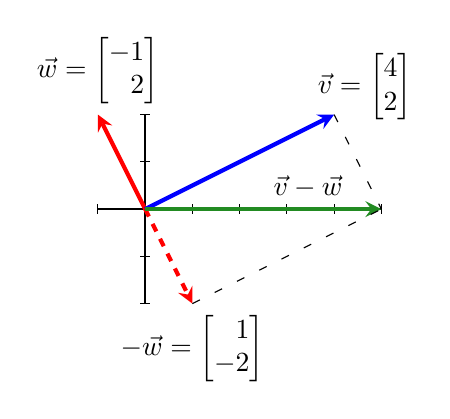
\begin{tikzpicture}[baseline,scale=0.6]
        \draw[] (-1,-0.1) grid (5,0.1);% x-ticks
        \draw[] (-0.1,-2) grid (0.1,2);
        \draw[semithick] (-1,0) -- (5,0);
        \draw[semithick] (0,-2) -- (0,2);
        \draw[line width=1.5pt,-stealth, red](0,0)--(-1,2) node[anchor=south,text=black]{$\vec{w} = \begin{bmatrix*}[r] -1\\ 2\\\end{bmatrix*}$};
        \draw[dashed,line width=1.5pt,-stealth, red](0,0)--(1,-2) node[anchor=north,text=black]{$-\vec{w} = \begin{bmatrix*}[r] 1\\ -2\\\end{bmatrix*}$};
        \draw[line width=1.5pt,-stealth,blue](0,0)--(4,2) node[xshift=-1em,yshift=1em, anchor=west,text=black]{$\vec{v} = \begin{bmatrix*}[r] 4\\ 2\\\end{bmatrix*}$};
        \draw[line width=1.5pt,-stealth, ForestGreen](0,0)--(5,0) node[xshift=-1em,anchor=south east,text=black]{$\vec{v} - \vec{w} $};
        \draw[loosely dashed](1,-2)--(5,0);
        \draw[loosely dashed](4,2)--(5,0);
    \end{tikzpicture}
\end{figure}

\tdplotsetmaincoords{60}{120}
\begin{tikzpicture}[tdplot_main_coords, scale=1.25]
    % Axes
    \draw [thick] (0,0,0) -- (2.25,0,0) node [below left] {$x$};
    \draw [thick] (0,0,0) -- (0,2.25,0) node [right] {$y$};
    \draw [thick] (0,0,0) -- (0,0,2.25) node [above] {$z$};
    % Ticks
    \foreach \i in {1,2}
    {
        \draw (\i,-0.1,0) -- ++ (0,0.2,0); % x
        \draw (-0.1,\i,0) -- ++ (0.25,0,0); % y
        \draw (0,-0.1,\i) -- ++ (0,0.2,0); % z
    }
    % vectors
    \draw[line width=1.5pt,-stealth, blue](0,0,0)--(2,2,0);
    \draw[line width=1.5pt,-stealth, red](0,0,0)--(0,2,1);       
    % Dashed lines
    \draw [dashed, blue]
        (2,0,0) -- (2,2,0) -- (0,2,0);
        % Dashed lines
    \draw [dashed, red]
        (0,2,0) -- (0,2,1) -- (0,0,1);
\end{tikzpicture}

\begin{tikzpicture}[tdplot_main_coords, scale=1.25]
    % Axes
    \draw [thick] (0,0,0) -- (2.25,0,0) node [below left] {$x$};
    \draw [thick] (0,0,0) -- (0,2.25,0) node [right] {$y$};
    \draw [thick] (0,0,0) -- (0,0,3.25) node [above] {$z$};
    % Ticks
    \foreach \i in {1,2}
    {
        \draw (\i,-0.1,0) -- ++ (0,0.2,0); % x
        \draw (-0.1,\i,0) -- ++ (0.25,0,0); % y
    }
    % Ticks
    \foreach \i in {1,2,3}
    {
        \draw (0,-0.1,\i) -- ++ (0,0.2,0); % z
    }
    % vectors
    \draw[line width=1.5pt,-stealth, blue](0,0,0)--(2,2,3);
    % Dashed lines
    \draw [dashed, blue]
        (2,0,0) -- (2,2,0) -- (0,2,0);
    \draw [dashed, blue]
        (0,0,3) -- (2,0,3) -- (2,2,3) -- (0,2,3) -- cycle;
    \draw [dashed, blue]
        (2,0,0) -- (2,0,3);
    \draw [dashed, blue]
        (2,2,0) -- (2,2,3);
    \draw [dashed, blue]
        (0,2,0) -- (0,2,3);
\end{tikzpicture}

\afterpage{\blankpage}


\end{document}